\section{Results}
\label{sec:2.2_results}

% 2.2.1
% -----
\subsection{Negative bias potential enhances signal in routine EM samples}

We first illustrate how the use of a potential bias can improve signal collection in a typical SEM experiment. A potential bias of \SI{-1}{\kilo\volt} is applied to the stage of an SEM with an integrated fluorescence microscope (Figure \ref{fig:2.1_setup}A \& B). The bias is applied via an external power supply connected to a custom stage plate such that the sample is electrically isolated from the rest of the fluorescence microscope and electrical components of the stage \cite{vos2021retarding}. By generating an electric field between the sample and the BSE detector, the bias potential accelerates signal electrons inwards away from their otherwise linear trajectories. Because of their lower energy, secondary electrons (<\,\SI{50}{\electronvolt}) are redirected inside the inner annulus of the BSE detector, while higher energy backscattered electrons (>\,\SI{50}{\electronvolt}) are redirected over a wider area depending on their initial emission angle and energy.

Pancreas tissue was prepared for integrated fluorescence-electron microscopy as described in Section \ref{sec:2.4.2_sampleprep}. No post-staining was applied resulting in lower contrast relative to other EM sample preparation protocols \cite{kuipers2015scanning}. EM images of EPON-embedded, \SI{80}{\nano\meter} tissue were acquired in immersion mode with and without a \SI{-1}{\kilo\volt} bias potential (Figure \ref{fig:2.1_setup}A \& B). When subject to a bias potential, EM images demonstrate noticeably higher contrast and less noise (Figure \ref{fig:2.1_setup}C \& G). The primary beam energy was increased by \SI{1}{\kilo\volt} such that the landing energy was held constant at \SI{1.5}{\kilo\electronvolt} in accordance with the section thickness. Data acquired with increased primary energy but without the use of stage bias (Figure \ref{fig:2.1_setup}D) reveals that the increase in apparent signal does not arrive solely from an increased primary energy. Moreover, the importance of maintaining a sufficiently low landing energy becomes clear by the visible artefacts from the ITO-coated glass substrate that appear with higher energies. The \SI{0.4}{\nano\ampere} beam current and \SI{5}{\micro\second\per\pixel} dwell time are held constant in each acquisition. The gain of the BSE detector had to be decreased while applying the negative bias to prevent the detector from saturating.

% Figure 2.1 (setup)
% -----------------
\begin{figure}[!tbh]
    \centering
    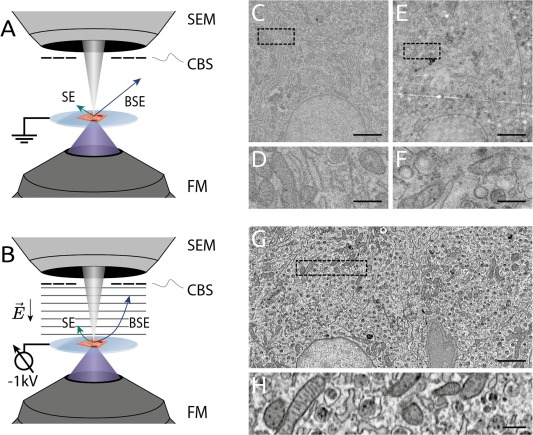
\includegraphics[width=\linewidth]{chapter-2/figures_JPEG_LQ/fig2-1_setup.jpg}
    \caption{Negative bias potential significantly enhances EM contrast in tissue. Schematic of integrated microscope without (A) and with (B) an applied stage bias. Electric field induced by the bias potential accelerates electrons emitted from the sample to the CBS detector. EM images of rat pancreas tissue without (C -- F) and with (G \& inset H) the use of stage bias. Biased images (G \& inset H) were acquired at \SI{2.5}{\kilo\electronvolt} primary energy with a \SI{-1}{\kilo\volt} bias potential---hence, a \SI{1.5}{\kilo\electronvolt} landing energy. For the sake of comparison, unbiased images (C \& inset D) were acquired with the same landing energy, while unbiased images (E \& inset F) were acquired with the same primary energy. The per-pixel dwell is held constant across all images at \SI{5}{\micro\second}. Vast improvement in EM signal and contrast can be seen by comparing insets (D \& F) with (H). Scale bars: \SI{2}{\micro\meter} (C, E, \& G); \SI{0.5}{\micro\meter} (D, F, \& H). Raw data at full resolution is available at \href{www.nanotomy.org}{Nanotomy}.}
    \label{fig:2.1_setup}
\end{figure}


% 2.2.2
% -----
\subsection{Simulating signal electron trajectories with and without negative potential bias}

% Figure 2.2 (simulations)
% ------------------------
\begin{figure}[!tbh]
    \centering
    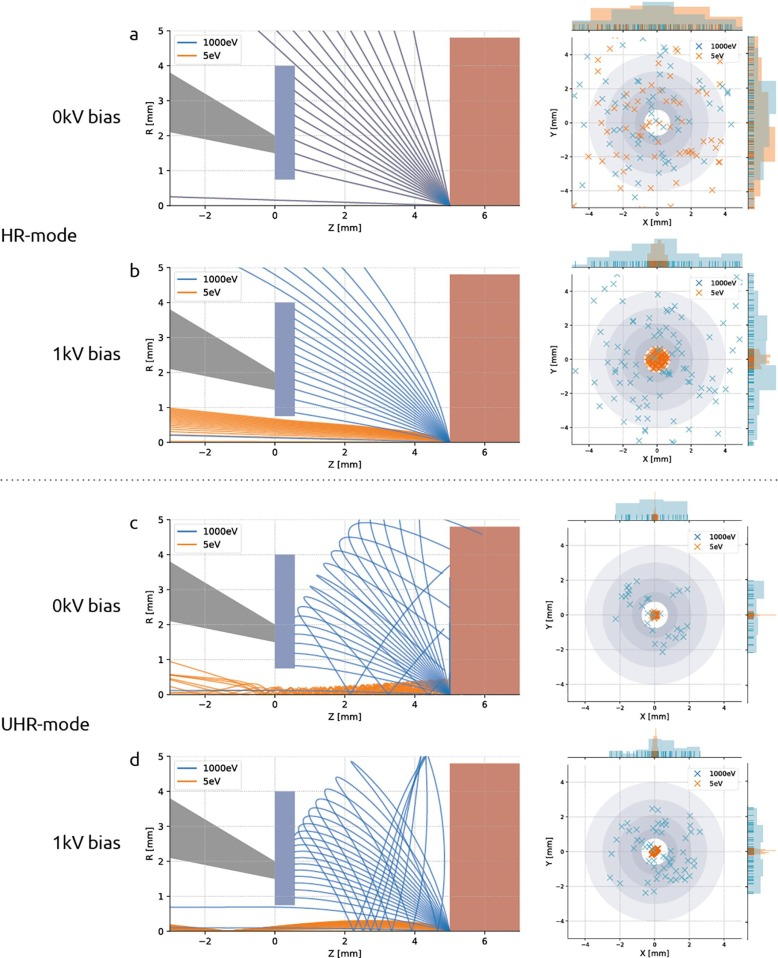
\includegraphics[width=0.85\linewidth]{chapter-2/figures_JPEG_LQ/fig2-2_simulations.jpg}
    \caption{Signal electron trajectories demonstrate the efficacy of stage bias in redirecting BSEs to the detector while simultaneously filtering out secondary electrons. Trajectory plots for SE and BSE bundles launched from the sample plane (left) and scatter plots (right) show the spatial distribution of signal electrons at the detector plane. In HR-mode, SEs and BSEs travel in overlapping, linear paths without the presence of an electric field (A), but BSEs get accelerated towards the detector when a negative bias potential is introduced (B). Signal electrons take on spiral trajectories in the presence of an immersion magnetic field (C), but are again steered to the detector when an electric field is added (D). In each set of simulations, BSEs (blue) and SEs (orange) are launched from the sample plane at $z =$ \SI{5}{\milli\meter}. Trajectory plots show geometry of the pole piece (grey), CBS detector (blue), and stage plate (red). Scatter plots show $x, y$ coordinates of signal electrons at the detector plane ($z =$ \SI{5}{\milli\meter}). Spatial distributions of signal electrons are plotted on the margins of the scatter plots.}
    \label{fig:2.2_simulations}
\end{figure}

Electron trajectories were simulated to better ascertain how a negative bias potential may give rise to better signal detection. Secondary electron and backscattered electron (BSE) trajectories were simulated for a variety of EM imaging conditions (Figure \ref{fig:2.2_simulations}). A model of the optical layout within the integrated microscope was developed in Electron Optical Design (EOD) \cite{lencova2008new} incorporating the geometry of the Verios 460 SEM objective lens and concentric backscatter (CBS) detector. The negative potential bias is factored into the model by implementing the sample plane as an additional lens element, which can then be biased to an arbitrary voltage. To mirror the \SI{5}{\milli\meter} working distance of our microscope, the end of the pole piece (grey element in Figure \ref{fig:2.2_simulations}) and start of the sample plane (red) are situated at $z=$ \SI{0}{\milli\meter} and $z=$ \SI{5}{\milli\meter} respectively. The roughly \SI{0.5}{\milli\meter} thick CBS detector (blue) is then located immediately below the pole piece.

Simulations were done for both non-immersion (high resolution or HR) and immersion (ultra-high resolution or UHR) SEM operation modes. For the case of non-immersion mode (Figure \ref{fig:2.2_simulations}A \& B), the magnetic focusing field is contained within the objective lens and therefore does not play a role in the signal electron trajectories. In these instances, the trajectories of the SEs and BSEs are dictated entirely by their initial velocity and the electric field due to the bias potential. In UHR-mode (Figure \ref{fig:2.2_simulations}C \& D), however, the sample is immersed in a strong magnetic field that both focuses the primary beam and---together with the electric field---alters the paths taken by the signal electrons. For this reason, the magnetic field strength is calculated by the field strength required to focus a parallel beam propagating in the $+z$ direction at the sample plane.

For each scenario shown, a bundle of secondary ($E_0 =$ \SI{5}{\electronvolt}) and backscattered electrons ($E_0 =$ \SI{1}{\kilo\electronvolt}) is emitted from the origin at $z =$ \SI{5}{\milli\meter}. The angular distribution is given by Lambert's cosine distribution \cite{reimer1998emission}. A screen is placed at the detector plane to record the radial position of the signal electrons, from which the scatter plots are generated (Figure \ref{fig:2.2_simulations}). The grey rings of varying diameter represent the individual segments of the CBS detector. For the case of non-immersion mode and no potential bias (Figure \ref{fig:2.2_simulations}A), the region between the detector and sample planes is field-free and the signal electrons travel freely in straight paths coinciding with one another. Only when a bias potential is added (Figure \ref{fig:2.2_simulations}B) do the higher energy BSEs diverge from the secondaries, which, due to their low initial energy, are accelerated inside the BSE detector before they are able to spread out radially. The trajectories change when under the influence of a magnetic immersion field (Figure \ref{fig:2.2_simulations}C) in which case the Lorentz force causes the signal electrons to spiral about the optical axis \cite{mullerova2009collection}. The low energy SEs remain tightly coiled as they propagate up through the BSE detector while the higher energy BSEs stretch out over greater radial distances. Whether the BSEs collide into the detector depends largely on the emission angle. The addition of a \SI{1}{\kilo\volt} bias potential (Figure \ref{fig:2.2_simulations}D) enables BSEs with a wider distribution of emission angles to reach the detector, resulting in the collection of more signal. These results suggest no secondary electron is ever registered as a count by the BSE detector---either because it is accelerated inside the detector or (in the field-free case) because it is of too little energy to generate an electron-hole pair \cite{vsakic2011boron}.

The collection efficiency of BSEs increases monotonically with increasing negative bias potential for both imaging modes (Figure \ref{fig:2.S1_percentages}). These results agree with what is suggested by the trajectory plots of Figure \ref{fig:2.2_simulations}---that the electric field generated by the stage bias tapers the radial spread of the BSEs leading to a greater percentage of BSEs collected. Note that the percentage of BSEs detected is greater for HR-mode across the range of bias potentials simulated. It therefore seems advantageous to prefer non-immersion mode, however, greater collection efficiency is only one factor to consider. The magnetic immersion field results in lower aberrations, meaning that for high resolution imaging, UHR mode is still often favourable. While the geometry modelled here is specific to our particular electron microscope, simulations were extended over a range of working distances and were found to follow the same general trends.% The electron trajectory data included in the supplemental data allows a user to input a range of working distances to simulate what BSE collection efficiency they might experience with their setup. Table \ref{} lists the available parameter space in which it is possible to trace BSE trajectories. Code for calculating the radial position of individual BSEs at a given detector plane is available within the supplemental material (Appendix \ref{}).


% 2.2.3
% -----
\subsection{Experimental optimization of negative potential bias leads to increased throughput}

EM imaging was expanded to encompass a wider imaging parameter space across a sequence of dwell times and negative bias potentials for both immersion and non-immersion mode based on the simulations (Figure \ref{fig:2.3_matrices}). The primary beam energy was increased together with the bias potential to hold the landing energy constant at \SI{1.5}{\kilo\electronvolt}. Likewise, the gain of the CBS detector was adjusted with each bias potential to keep the intensity levels from clipping. The detector gain and offset were manually calibrated to acquire over the full 16-bit range of the detector. This was not always possible, however, as many of the images acquired with low or no bias potential took up only a fraction of the detector's bandwidth, even at maximum gain.

% Figure 2.3 (matrices)
% ---------------------
\begin{figure}[!tbh]
    \centering
    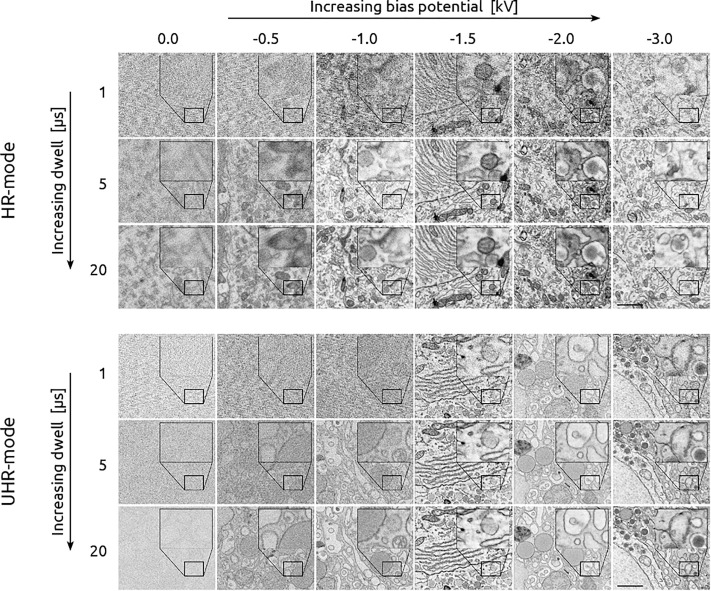
\includegraphics[width=\linewidth]{chapter-2/figures_JPEG_LQ/fig2-3_matrices.jpg}
    \caption{Negative bias potential delivers 5--20 times faster imaging while maintaining image quality. Bias potential varies from \SIrange[range-phrase=\text{ to }]{0}{-3}{\kilo\volt} (left to right) while the integration time varies from \SIrange[range-phrase=\text{ to }]{1}{20}{\micro\second} (top to bottom) for both the non-immersion (top) and immersion mode (bottom) image matrices. All images acquired with \SI{1.5}{\kilo\electronvolt} landing energy to match penetration depth. Scale bars: \SI{1}{\micro\meter}. Raw data is available at \href{www.nanotomy.org}{Nanotomy}.}
    \label{fig:2.3_matrices}
\end{figure}

An increase in image signal with increasing negative bias potential for both imaging modes up to roughly \SI{-1500}{\volt} was recorded (Figure \ref{fig:2.3_matrices}), after which it becomes difficult to perceive notable differences in image quality. The signal appears to improve more gradually in non-immersion mode, whereas the improvement for immersion mode is more abrupt. Furthermore, in certain instances, increasing the integration time by several factors results in a less substantial increase to the apparent SNR than a \SI{500}{\volt} increase to the negative bias potential. This is significant as the integration time is typically the primary imaging parameter to improve image quality—and large increases come at the direct expense of throughput.

Quantitative SNR measurements, based on the spectral signal-to-noise ratio (SSNR) \cite{unser1987new}, were made on the collection of images and averaged for each combination of bias potential, dwell, and imaging mode (Figure \ref{fig:2.4_snr}). These measurements were corroborated using a separate cross-correlation-based SNR method \cite{joy2002smart} (Figure \ref{fig:2.S2_comparison}). In particular, these measurements reveal that an image acquired in non-immersion mode with a \SI{1}{\micro\second} dwell time and \SI{-1.5}{\kilo\volt} bias potential yields roughly the same SNR as an image acquired with a \SI{5}{\micro\second} dwell but with no applied bias. The effect of the potential bias is even more pronounced in immersion mode where the SNR of a \SI{1}{\micro\second} image with a \SI{1.5}{\kilo\volt} stage bias exceeds that of a \SI{20}{\micro\second} image acquired without a bias. Fourier analysis was done to analyse the effect of the bias potential in different frequency domains (Figure \ref{fig:2.5_noise}). The center spot of the 2D FFTs—containing most of the signal—becomes more prominent with increasing bias potential. This growth is reflected in the SSNR spectra, which show order of magnitude increases in amplitude in the low spatial frequency domain. Furthermore, the high frequency streak artefacts present in the lower bias potential images---visible in the 2D FFTs---become suppressed at higher bias potentials.

% Figure 2.4 (SNR)
% ----------------
\begin{figure}[!tbh]
    \centering
    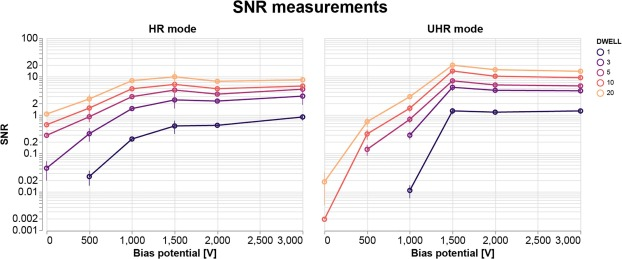
\includegraphics[width=\linewidth]{chapter-2/figures_JPEG_LQ/fig2-4_snr.jpg}
    \caption{Optimization of bias potential delivers SNR increases of multiple orders of magnitude. At bias potentials greater than \SI{1.5}{\kilo\volt}, the SNR is found to level off for both imaging modes. Images are comprised of varying stage bias potentials, integration times, and imaging modes but with fixed \SI{1.5}{\kilo\electronvolt} landing energy and \SI{5}{\milli\meter} working distance. Different color lines represent different dwell times as indicated by the legend. SNR measurements are averaged over five EM images at different areas of the tissue for each combination of bias potential, dwell time, and imaging mode. Error bars indicate the standard deviation in the SNR over the five images. Missing data points indicate a negative SNR, which may occur for images with extremely high noise.}
    \label{fig:2.4_snr}
\end{figure}


% Figure 2.5 (noise)
% ------------------
\begin{figure}[!tbh]
    \centering
    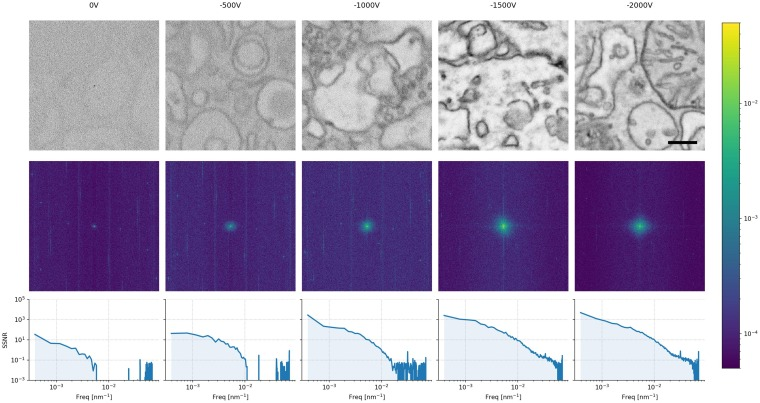
\includegraphics[width=\linewidth]{chapter-2/figures_JPEG_LQ/fig2-5_noise.jpg}
    \caption{Noise contributions suspected to originate from the scanning electronics are suppressed with increasing bias potential. Top: sequence of \SI{5}{\micro\second} dwell tissue images acquired in immersion mode with varying amounts of stage bias. Center: 2D FFTs of tissue images showing the central spot, which represents most of the signal, becoming more prominent with increasing bias potential up to \SI{-1.5}{\kilo\volt}. The 2D FFTs exhibit noticeable streak artefacts at higher frequencies, particularly in the lower bias potential images. We attribute these streaks to electric interference from the scanning electronics. Furthermore, there is a constant offset, which is likely a combination of shot noise from various sources, and may also include a component from the scanning electronics. Bottom: SSNR spectra show a division between the low frequency (primarily signal) and high frequency (primarily noise) portions of the tissue images. As the suspected scanning electronics noise is drowned out, the SNR improves dramatically. Scale bar: \SI{500}{\nano\meter}.}
    \label{fig:2.5_noise}
\end{figure}


% 2.2.4
% -----
\subsection{Potential bias allows for higher throughput EM and CLEM acquisitions}

Only small regions of interest are typically recorded at high resolution EM given that full section imaging at sub-\SI{10}{\nano\meter} resolution often takes an excessive amount of time. As a result of the enhanced signal-to-noise ratio afforded to us by the use of a negative bias potential, we are able to significantly expedite the imaging of a thin section of HeLa cells at \SI{5}{\nano\meter} resolution (Figure \ref{fig:2.6_cells}). Based on our empirical results (Figure \ref{fig:2.4_snr}), a negative potential bias of \SI{-1.5}{\kilo\volt} was chosen for EM imaging in immersion mode. A per-pixel dwell time of \SI{2}{\micro\second} was chosen to balance high SNR and image clarity with overall imaging time. Control images of the same cell were acquired without the use of a bias potential at the same landing energy (Figure \ref{fig:2.6_cells}A) and primary energy (Figure \ref{fig:2.6_cells}B). The total imaging time for this \SI{550}{\micro\meter} $\times$ \SI{350}{\micro\meter} area was \SI{5.6}{\hour}.

% Figure 2.6 (cells)
% ------------------
\begin{figure}[!tbh]
    \centering
    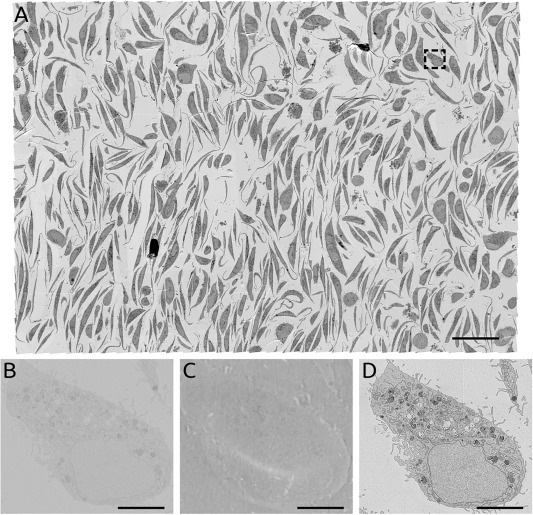
\includegraphics[width=\linewidth]{chapter-2/figures_JPEG_LQ/fig2-6_cells.jpg}
    \caption{Fast, high resolution EM gigapixel image of cultured cells. (A) EM acquisition of a \SI{100}{\nano\meter} section of HeLa cells as a nanotomy map. Section imaged at \SI{1.5}{\kilo\electronvolt} LE and with a \SI{-1.5}{\kilo\volt} bias potential. For the sake of comparison, one HeLa cell was acquired at multiple energy settings: (B) \SI{1.5}{\kilo\electronvolt} LE with no bias potential; (C) \SI{3}{\kilo\electronvolt} LE with no bias potential; (D) \SI{1.5}{\kilo\electronvolt} LE with \SI{-1.5}{\kilo\volt} bias potential—identical to that of the large-scale acquisition. Scale bars: \SI{50}{\micro\meter} (A); \SI{5}{\micro\meter} (B, C, \& D). Raw data is available for viewing via \href{www.nanotomy.org}{Nanotomy}.}
    \label{fig:2.6_cells}
\end{figure}

To demonstrate the application of a negative bias potential on samples also prepared for immunofluorescence, a large-scale acquisition was conducted on a section of rat pancreas tissue (Figure \ref{fig:2.7_rat}). Full section (\SI{0.5}{\milli\meter^2}) acquisition including fluorescence imaging, stage translations, and additional overhead factors was completed in \SI{8}{\hour}. Table \ref{tab:2.1_timing} provides an overview of the time spent on each aspect of the workflow, and exemplifies the potential time savings afforded by using a bias potential. We note that no post-staining was applied to this section in order to allow integrated acquisition of fluorescence for high-precision overlaid FM. Fluorescence images were acquired prior to EM to prevent quenching of the fluorescence due to electron beam irradiation. The insulin-producing beta cells---clustered within the islet of Langerhans---were immunolabelled and given a Hoechst counterstain to target cell nuclei as well as the rough endoplasmic reticulum in the exocrine region of the tissue (blue) (Figure \ref{fig:2.7_rat}A). The section edges can easily be discerned from the FM images, facilitating the area selection for subsequent EM imaging (Figure \ref{fig:2.7_rat}B). Here the islet (light grey region) can be seen surrounded by the exocrine tissue (dark grey). An automated registration procedure \cite{haring2017automated} was done to overlay the fluorescence signal onto the EM images (Figure \ref{fig:2.7_rat}C) such that the fluorescence signal is correlated at high resolution across the entire EM field of view (Figure \ref{fig:2.7_rat}D \& E). Additional details of how the correlative acquisition and reconstruction were done are provided in Sections \ref{sec:2.4.4_workflow} and \ref{sec:2.4.5_reconstruction} respectively.

% Figure 2.7 (rat)
% ----------------
\begin{figure}[!tbh]
    \centering
    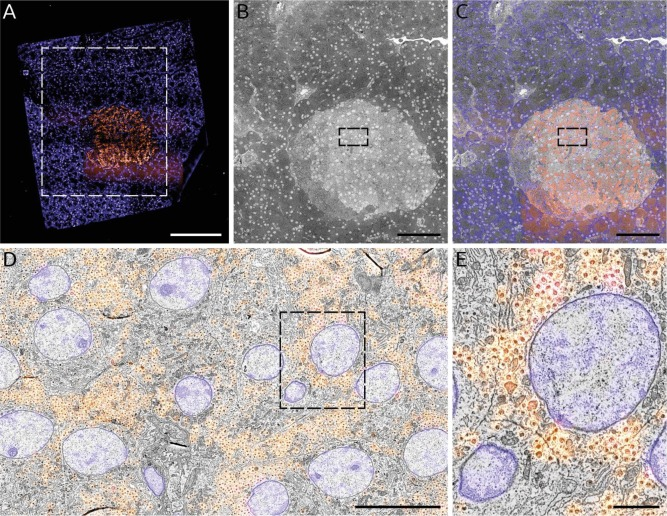
\includegraphics[width=\linewidth]{chapter-2/figures_JPEG_LQ/fig2-7_rat.jpg}
    \caption{Fast, correlative imaging of a complete EM section at high resolution. \SI{80}{\nano\meter} rat pancreas tissue was imaged at \SI{3}{\kilo\electronvolt} beam energy with a \SI{-1.5}{\kilo\volt} stage bias (\SI{1.5}{\kilo\electronvolt} landing energy) with \SI{2}{\micro\second} dwell as a nanotomy map. (A) Composite two-channel FM image of the tissue section: cell nuclei (blue) stained by Hoechst; insulin-producing beta cells (orange) immunolabeled with Alexa 594. (B) Composite EM image of the area outlined in (A) comprising the islet of Langerhans identified via FM imaging. (C) Correlative overlay of the islet and surrounding exocrine tissue. (D) Zoomed-in area of islet outlined in (B \& C) with inset (E) exhibiting the native resolution (\SI{5}{\nano\meter} pixel size) that exists across the entirety of the nanotomy map. Total imaging time is \SI{8}{\hour}, the majority of which is taken up by the high-resolution EM imaging. Note that a similar area at this pixel size (see e.g. \textcite{ravelli2013destruction}) typically takes upwards of \SI{24}{\hour} with TEM. Scale bars: \SI{200}{\micro\meter} (A); \SI{100}{\micro\meter} (B \& C); \SI{10}{\micro\meter} (D); \SI{2}{\micro\meter} (E). Raw data is available via \href{www.nanotomy.org}{Nanotomy}.}
    \label{fig:2.7_rat}
\end{figure}


% Table 2.1 (timing)
% ------------------
\begin{table}[!tbh]
    \centering
    \caption{Use of optimized potential bias leads to an 80\% reduction in total imaging time for a typical large-scale acquisition. The total imaging time is highly dependent on the ROI size, which may vary widely depending on the biological application. Here the typical diameter of an islet of Langerhans is given, while in Figure \ref{fig:2.7_rat} a \SI{700}{\micro\meter} $\times$ \SI{700}{\micro\meter} area was chosen as the ROI—resulting in the \SI{8}{\hour} total acquisition time. Total imaging times for arbitrary ROI sizes can be determined by first calculating the number of image tiles needed: $N=\text{ceil}\left((L-ow) - (w-ow)\right)^2$ where $L$ is the typical section or ROI width, $o$ is the percentage overlap between image tiles, and $w$ is the field of view. Note that the negative overlap given for the low-magnification CLEM tiles reflects that these tiles do not overlap with one another.}
    \footnotesize
    \begin{tabular}{@{}p{15mm}p{30mm}rrrr@{}}
    \toprule
    \multicolumn{1}{r}{} & \multicolumn{1}{r}{} & \multicolumn{2}{c}{\textbf{Low-mag CLEM}} & \multicolumn{2}{c}{\textbf{Hi-mag EM}} \\
     \arrayrulecolor{black!30}\cmidrule(l){3-4} \cmidrule(l){5-6}
     &  & \textbf{No bias} & \textbf{Bias} & \textbf{No bias} & \textbf{Bias} \\
     \arrayrulecolor{black!30}\midrule
     & Pixel size & 36.6 nm &  & 4.88 nm &  \\
     & Dwell & 10 µs & 2 µs & 10 µs & 2 µs \\
     & Field of View & 150 µm &  & 20 µm &  \\
     & Overlap (b/w images) & −36 µm (−24\%) &  & 2.4 µm (12\%) &  \\
     & N. pixels & 16.8 Mpx &  & 16.8 Mpx &  \\
    \multirow{-6}{*}{EM} & Acquisition time & 168 s & 33.6 s & 168 s & 33.6 s \\
    \arrayrulecolor{black!30}\midrule
     & Exposure time & 5 s &  &  &  \\
     & N. channels & 2 &  &  &  \\
    \multirow{-3}{*}{FM} & Acquisition time & 10 s &  &  &  \\
    \arrayrulecolor{black!30}\midrule
     & Registration procedure & 20 s &  &  &  \\
    \multirow{-2}{*}{Overhead} & Stage translation & 4 s &  & 2 s &  \\
    \arrayrulecolor{black!30}\midrule
    Total & Total acquisition time (per CLEM/EM image) & 202 s & 68 s & 170 s & 36 s \\
    \arrayrulecolor{black}\midrule
    \rowcolor[HTML]{E8E8E8} 
    \cellcolor[HTML]{E8E8E8} & Typical size & 700 µm &  & 250 µm &  \\
    \rowcolor[HTML]{E8E8E8} 
    \cellcolor[HTML]{E8E8E8} & N. image tiles & 16 &  & 225 &  \\
    \rowcolor[HTML]{E8E8E8} 
    \multirow{-3}{=}{\cellcolor[HTML]{E8E8E8}Large-scale acquisition} & Total acquisition time & 54 min & 18 min & 11 hr & 133 min \\
    \bottomrule
    \end{tabular}
    \label{tab:2.1_timing}
\end{table}
